\chapter{Evaluation}\label{chap:evaluation}

Neither persistent base nodes nor snapshotting lead to direct performance
benefits for Soup. Instead, they both come with a wide range of features and
improvements in other areas, helping Soup make a significant leap towards being
a production-ready database system. Moving the base node state to durable
storage lets Soup operate on datasets larger than its memory size, while
reducing the overall memory usage of the system. It improves the system's
overall recovery capabilities---a necessity if Soup is ever going to be usable
for long running applications. Snapshotting takes this a step further, and
removes the performance penalty Soup sees while its partial states are brought
back to the state they were prior to a fatal failure.

Regardless, Soup's performance when faced with a large amount of concurrent
requests is still one of its main contributions. While a certain reduction in
throughput and latency might be inevitable, it is crucial that this penalty
remains as insignificant as possible. This chapter first investigates the
effects \code{PersistentState} has on performance, followed by a look at the
recovery benefits from both \code{PersistentState} and snapshotting.

\section{Write-performance}

Only a small subset of reads propagate all the way to the base nodes. Instead,
they are served by partially materialized nodes further down the graph, avoiding
the need for expensive computations on each read. This is not the case with
writes. Every update that reaches Soup needs to be fully persisted to durable
storage before a write acknowledgment can be sent. With persistent base nodes,
that involves materializing the updates into \code{PersistentState}. With
packets being processed synchronously at each domain, even the smallest increase
in write latency at the base nodes could have disastrous effects for the overall
write throughput of the system.

The \code{vote} benchmark described in section~\ref{sec:vote} is used to measure
write-performance. While it is normally a mixed-load benchmark where clients
both write new votes and read the existing vote counts of articles, we will run
\code{vote} with a pure write-load, removing reads altogether. Since we are
measuring the impact of writing to durable storage, Soup will run without
sharding, resulting in a single domain writing new votes to
\code{PersistentState}. The database is pre-populated with 100K articles and the
inserted votes are uniformly distributed across the existing articles.

Soup can be run both in a local and distributed fashion, and \code{vote}
supports both. Writing to durable storage is a penalty fixed per machine
however, and benchmarking the horizontal scalability makes little sense.
Instead, we will use the \textit{local} \code{vote} benchmark, where both the
clients and the Soup workers run on the same machine.

\begin{figure}[H]
  \centering
  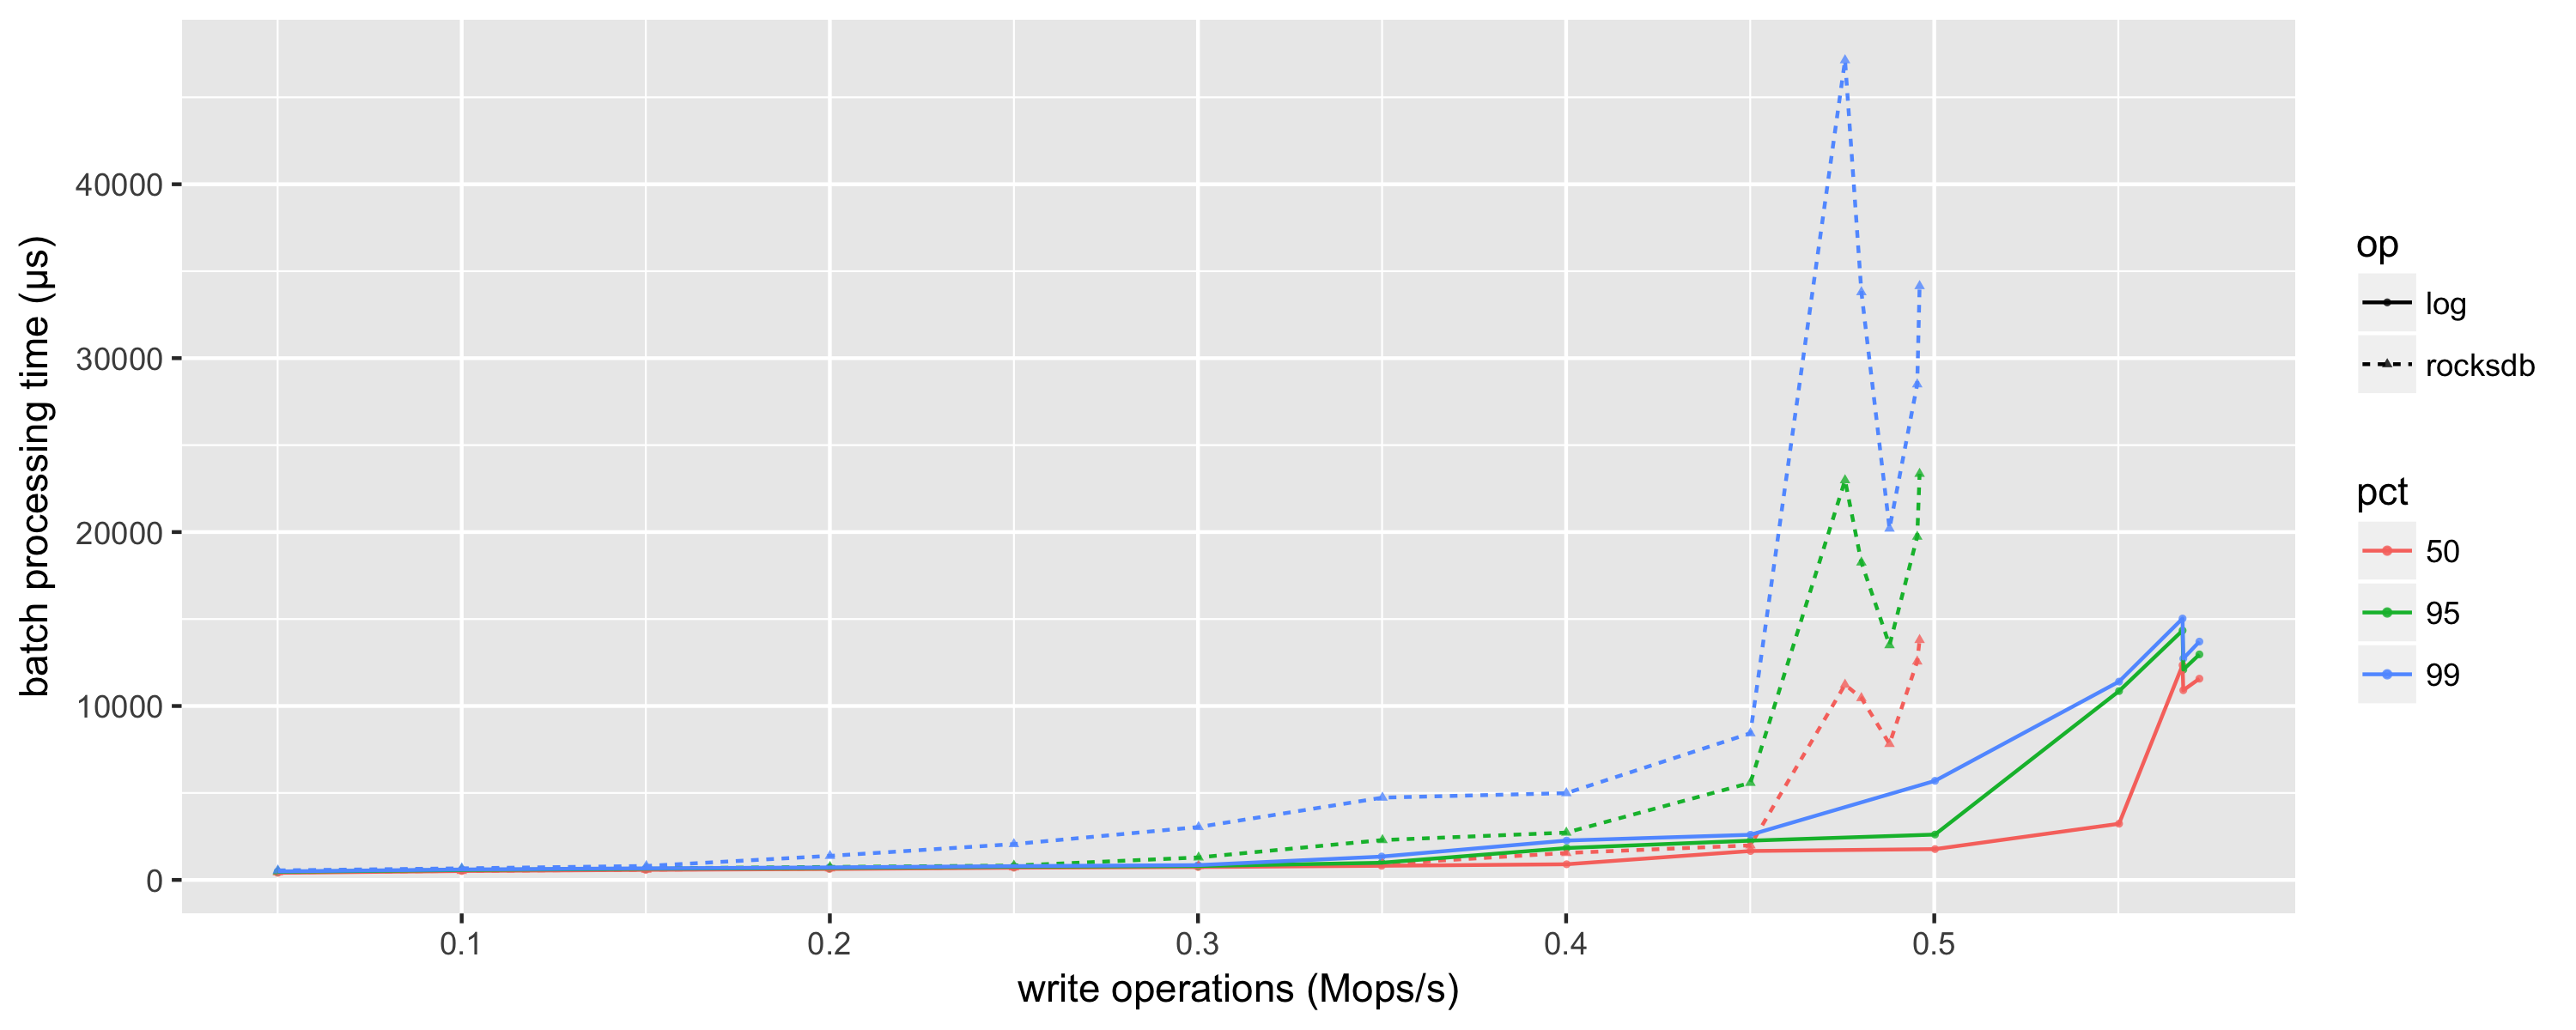
\includegraphics[width=\textwidth]{graphs/write-batch}
  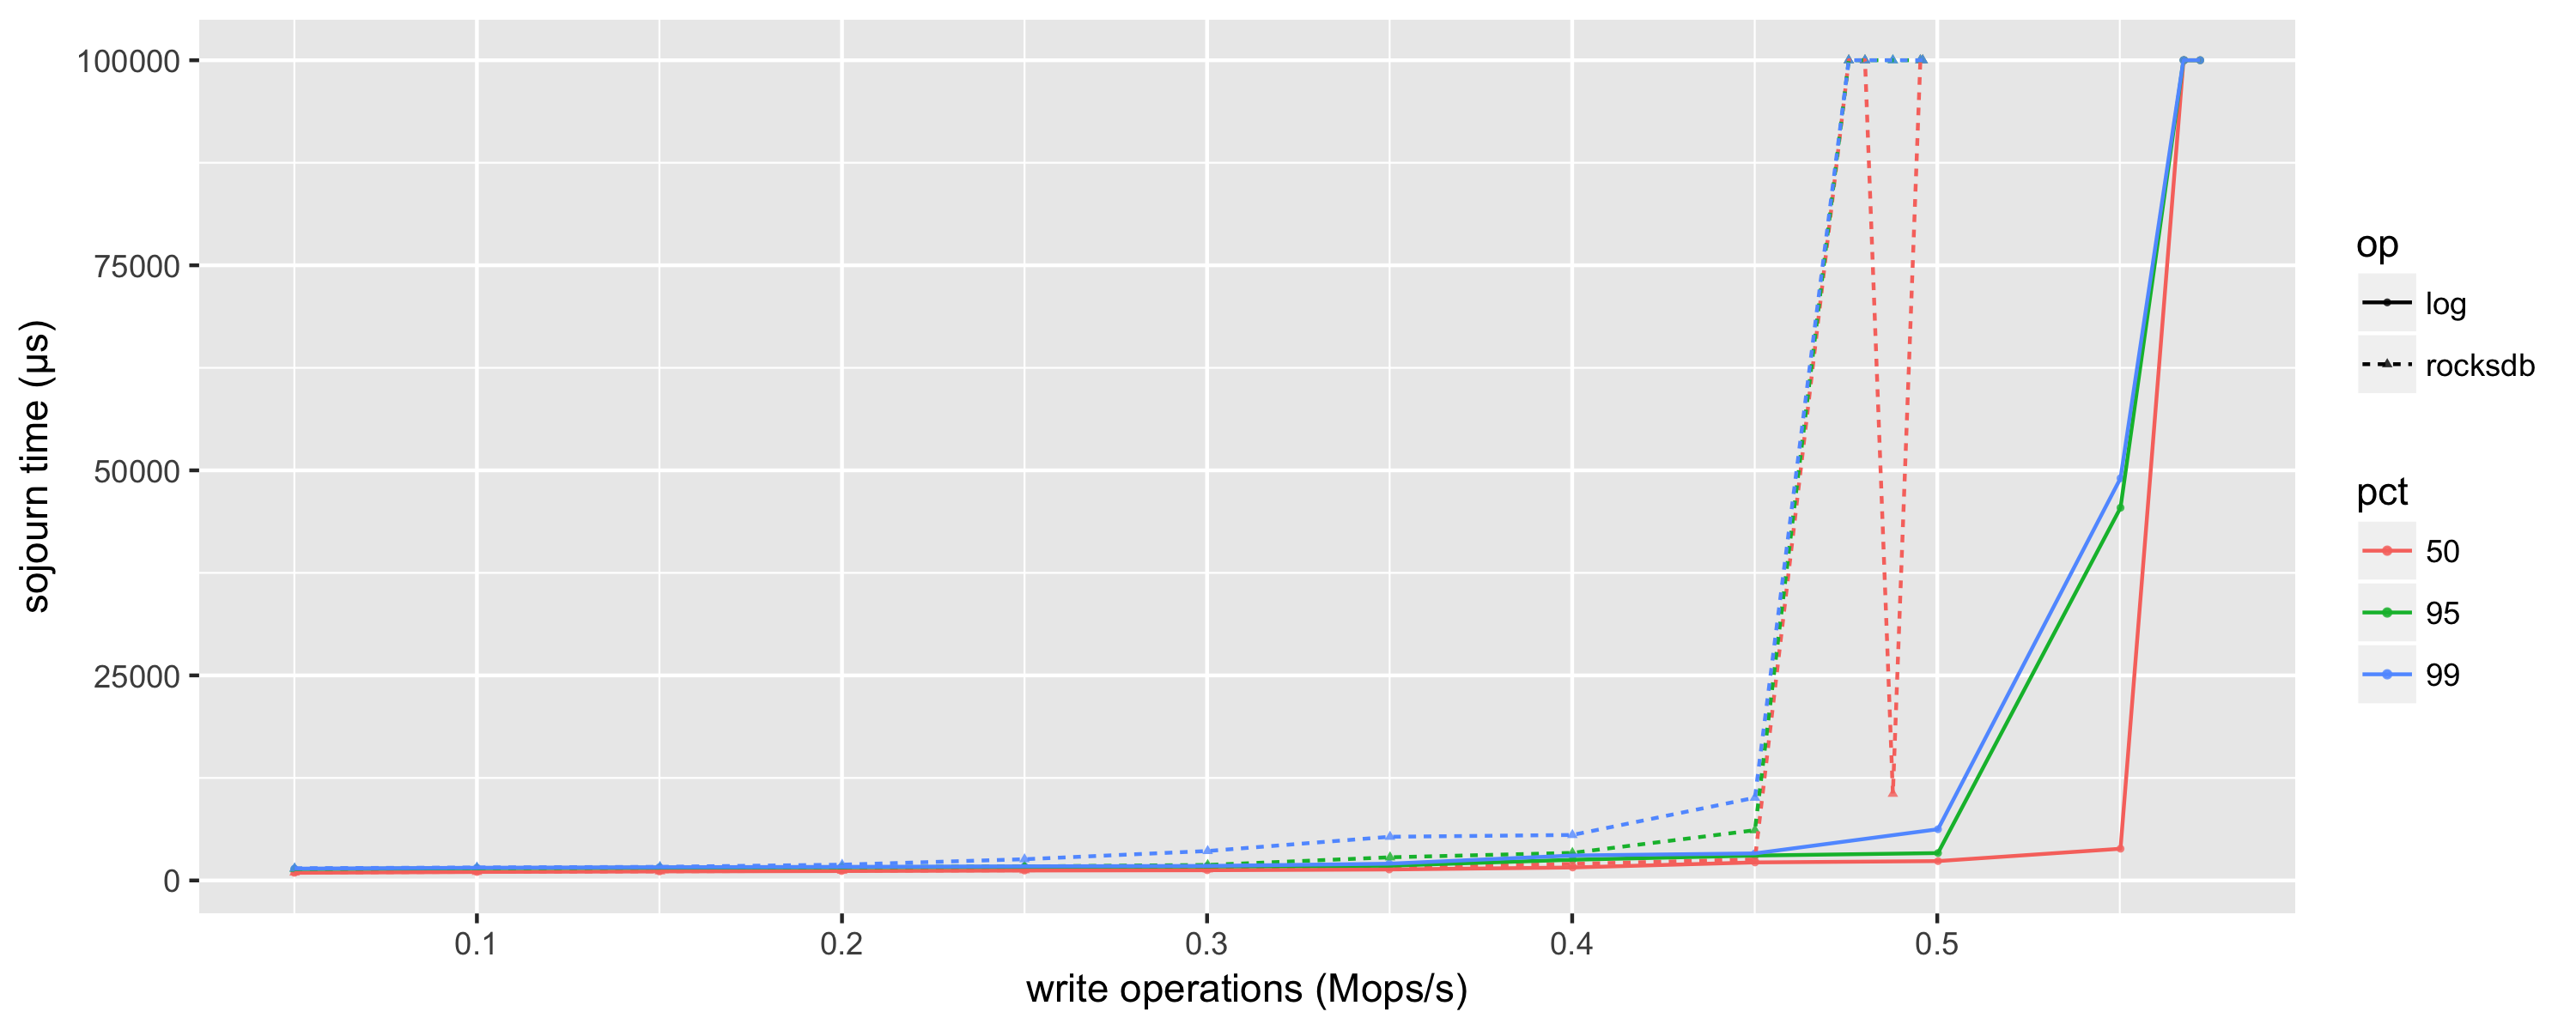
\includegraphics[width=\textwidth]{graphs/write-sjrn}
  \caption{\
    Write-only comparison of Soup's regular write-ahead log and RocksDB.\@
    TODO: describe batch/sojourn
  }\label{graph:write}
\end{figure}

\section{Read-performance}

When measuring the overall read-performance of Soup as a system, a read heavy
\code{vote} benchmark is a good indicator. To analyze the impact of persisting
state to durable storage at the base nodes we want to ensure that we are
actually measuring the read performance of the \textit{base nodes} however, and
not the partial nodes further down the graph. Instead, we will make use of the
replay benchmark described in section~\ref{sec:bench-replay}, where each row is
read at most once, resulting in a full replay from the base nodes.

The database is pre-populated with 10 million rows, after which a small random
subset of the rows are read once. With \code{PersistentState}, Soup recovers
existing data between each test run, after flushing the disk caches.

\begin{figure}[H]
  \centering
  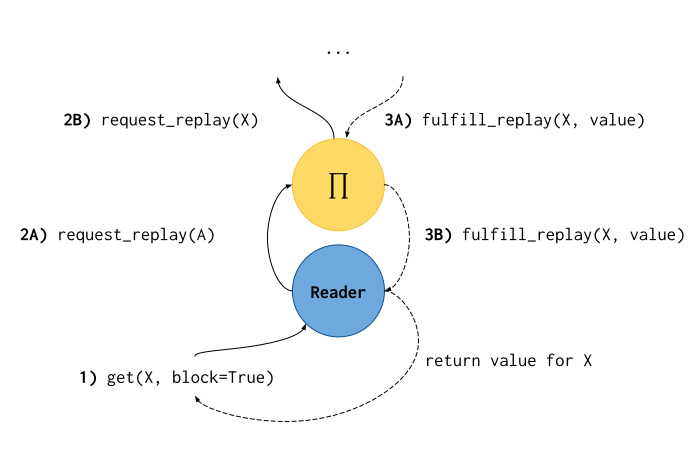
\includegraphics[width=\textwidth]{graphs/replay}
  \caption{\
    The replay performance of in-memory Soup compared to Soup with RocksDB.\@
  }\label{graph:replay}
\end{figure}

\subsection{SS-table format}

RocksDB provides two separate SS-table implementations, \code{BlockBasedTable}
and \code{PlainTable}.

\todo{write more!}

\begin{figure}[H]
  \centering
  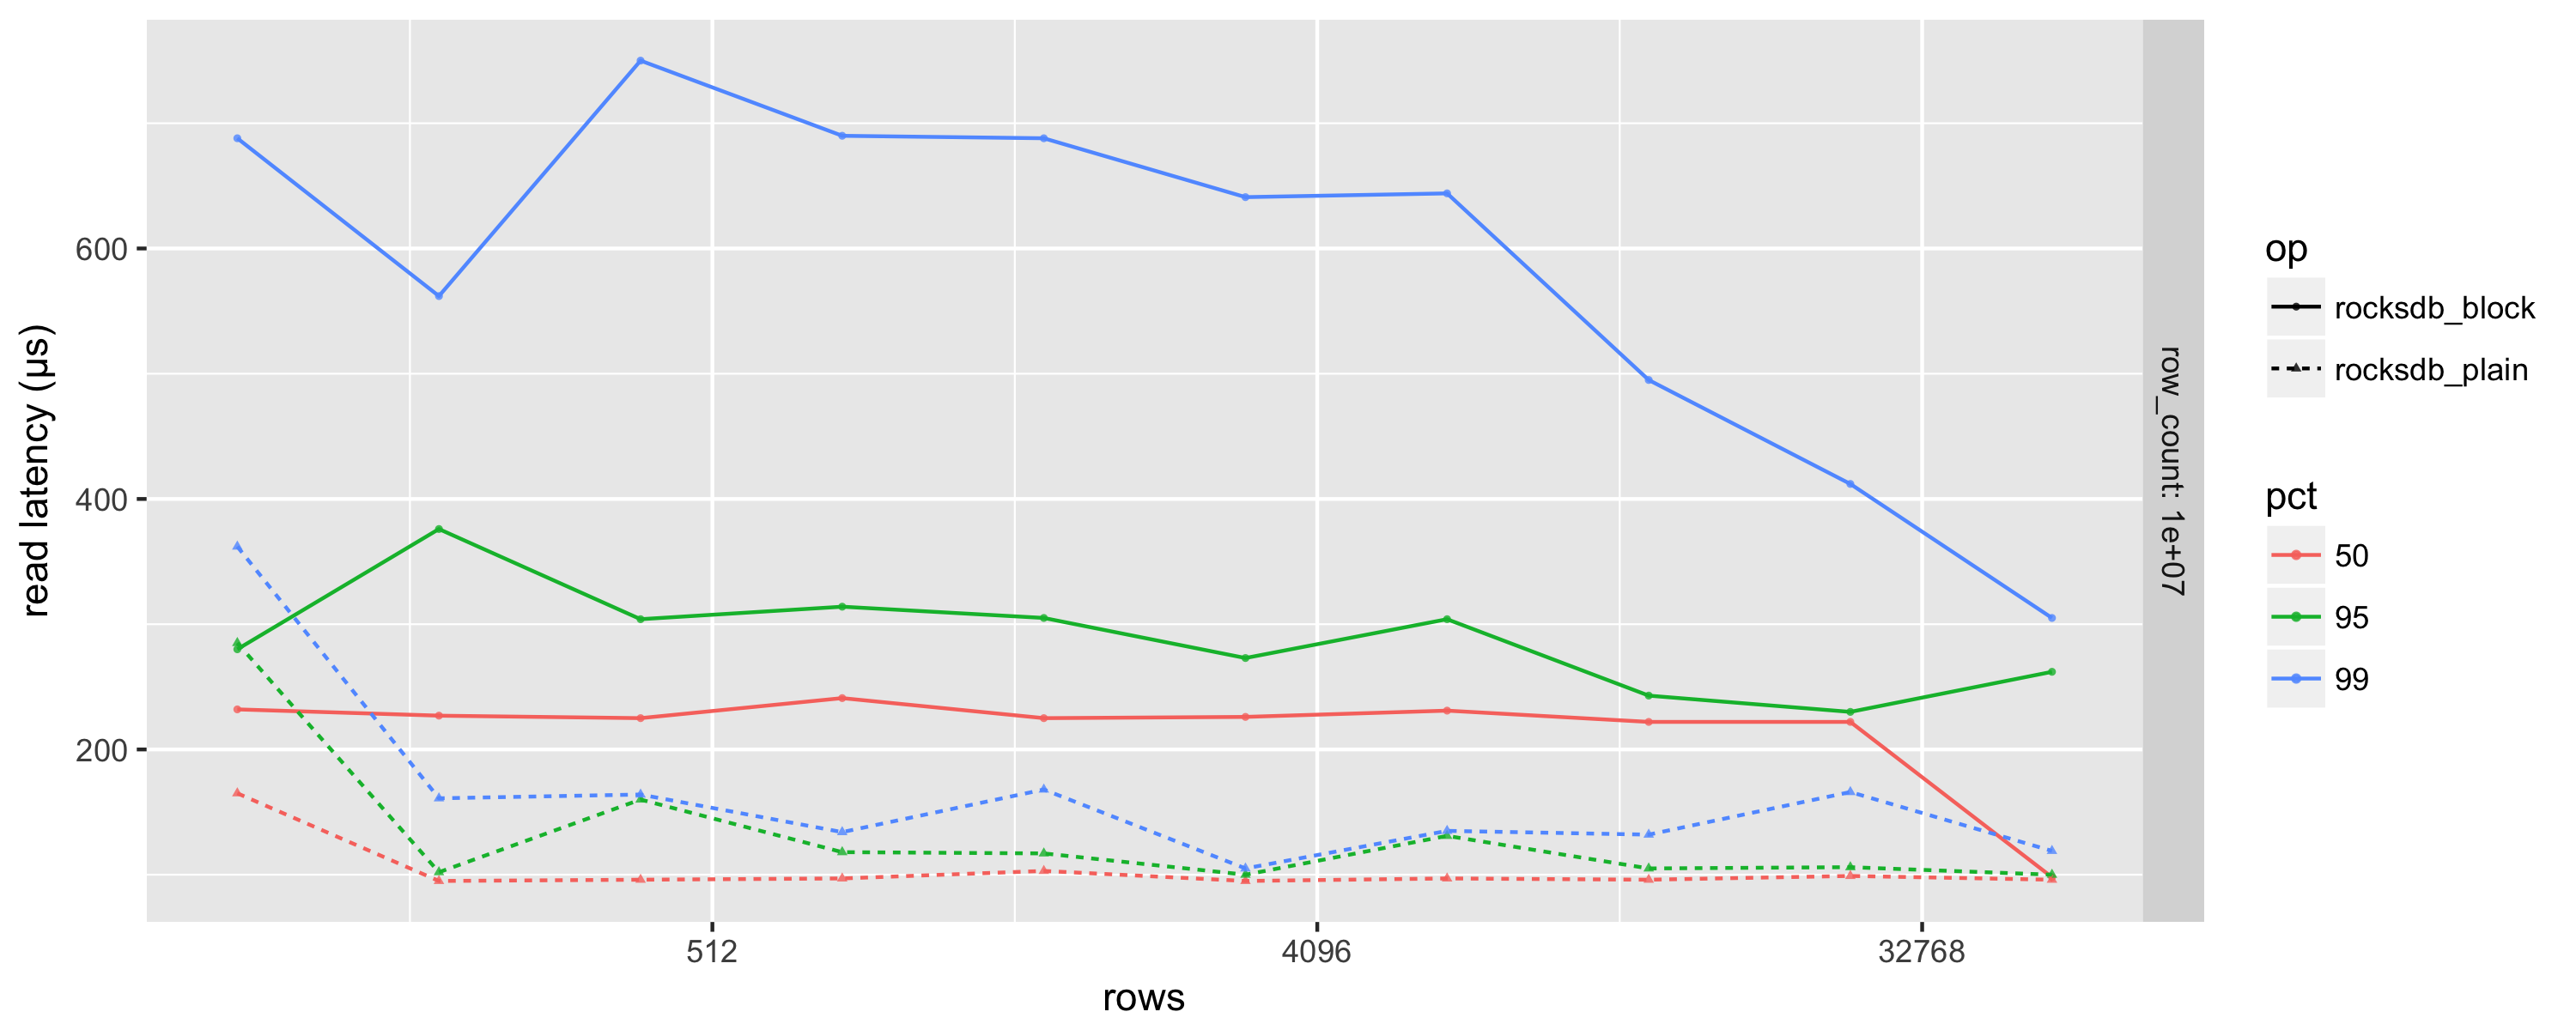
\includegraphics[width=\textwidth]{graphs/replay-table}
  \caption{\
    Soup replay performance comparison between \code{BlockBasedTable} and
    \code{PlainTable}.
  }\label{graph:replay-table}
\end{figure}



\section{Mixed workload}
\section{Recovery}
